\documentclass[main.tex]{subfiles}

\begin{document}
\section{Характеристики}
    \subsection{Избор}
    На дневен ред е избирането на характеристики, които отразяват идеята за разделяне на информацията за вокалния тракт
    $\mathcal{H}$ от входния сигнал $\mathcal{G}$.
    Имаме $\mathcal{Y}(\mathcal{z}) = \mathcal{G}(\mathcal{z}) \mathcal{H}(\mathcal{z})$.

    Нека вземем логаритъм от модула:
    \begin{flalign*}
        & log(|\mathcal{Y}(\mathcal{z})|) = log(|\mathcal{G}(\mathcal{z})|) + log(|\mathcal{H}(\mathcal{z})|) &&
    \end{flalign*}
    Обратното Фурие преобразувание ни дава вид във времевия домейн:
    \begin{flalign*}
        & c_y[n] = c_g[n] + c_h[n] &&
    \end{flalign*}

    Сега вече имаме сбор на входния сигнал и този на филтъра, вместо конволюция във времевия домейн.

    Да видим каква е идеята зад тези преобразувания.
    Имаме, че $\mathcal{G}(\mathcal{z})$ и $\mathcal{H}(\mathcal{z})$ са комплексни числа и взимайки модула им, губим информация за фазата. Това не е проблем, тъй като човешкото ухо не е особено чувствително към нея, затова обикновено ни трябва само амплитудата (и следователно модула). 
    
    \begin{figure}[H]%
        \centering
            \subfloat[Логаритмична скала]{%
                \label{fig:char:1:a}
                \includegraphics[width=0.40\paperwidth,valign=t]{aaaa.png}%
            }
            \hfill
            \subfloat[Логаритмична скала и логаритъм от модула]{%
                \label{fig:char:1:b}
                \includegraphics[width=0.40\paperwidth,valign=t]{aaaa_log.png}%
            }
        \caption{Графика на спектъра на сигнал, получен при произнасяне на "а-а-а-а-а"}%
        \label{fig:char:1}
    \end{figure}

    Взимането на логаритъм, подчертава периодичността на сигнала, идващ от глотиса. На Фигура \autoref{fig:char:1:a} се виждат пиковете, породени от
    фундаменталната честота, на която трепти глотиса, и хармоничните и честоти. Поради загубата на енергията в системата за производство на реч, не всички хармонични честоти имат същата амплитуда.
    На Фигура \autoref{fig:char:1:b} се вижда, че взимането на логаритъм помага за изравняването на хармоничните амплитудати и кара графиката да изглежда "по-периодична". Честотите на \autoref{fig:char:1} са изобразени върху логаритмична скала, вместо линейна, тъй като е емпирично установено, че ухото възприема звука логаритмично, но това ще бъде по-подробно разгледане в следващия подраздел.
    Сега нека разгледаме логаритмувания спектър като сигнал и му направим Фурие преобразувание до получаване на така нареченият кепстър.
    Тъй като разглеждаме спектъра сигнал, наличието на периодични амплитуди ще се преведе до пик в получения кепструм на честотата, отговаряща (горе-долу, имайки предвид джитера) на основната честота на глотиса. Информацията, която описва вокалния тракт е с много по-малко изразена периодичност в спектъра, затова ще се запази в ниските честоти на кепстъра. Тоест $c_g[n]$  ще са коефициентите в кепстъра на високите честоти, а $c_h[n]$ в ниските. За практически цели обикновено се избират първите 13 коефициента на кепстъра. Тези коефициенти се наричат Mel Frequency Cepstral Coefficients (MFCC), където Mel скалата е логаритмична скала. Повече детайки за извличането им са описани в следващия подраздел.

    \subsection{Извличане}
    Ще извличаме характеристики от подаден аудио файл в wave формат. Първо, съдържанието на файла се прочита в масив от 64-битови float числа. Елементите на този масив се наричат дискрети (samples). Броят им зависи от честотата на дискретизация (тоест колко измервания са направени за една секунда), която обикновено е 16kHz, 44100Hz или 48Hz. Броят на дискретите определя броя на коефициентите на Фурие преобразуванието. Тъй като сигналът е реален, от \hyperref[appendix:fourier:property]{свойствата} следва, че максималната честота, която можем да измерим е честотата на Найкуист, равна на броя дискрети върху две, тоест половината на честотата на дискретизация.
    Колкото е по-голяма Найкуист честотата, толкова по-добра честотна резолюция получаваме.\\
    Базирайки се на идеята, че вокалният тракт е статичен за кратък период от време, накъсваме масива отделни застъпващи се парчета - фреймове - в рамките на които сигналът е статичен. За да се определи дължината на фрейма, трябва да се вземат предвид две неща: от една страна колкото повече дискрети имаме, толкова по-добра честотна резолюция получаваме. От друга, колкото повече данни взимаме, толкова по-голям е шансът да се смени конфигурации на вокалния тракт. За да се справим с този дуализъм, компромисните стойности, които са избрани в описваната имплементация, са 25 милисекунди за дължина на фрейм и 10 милисекунди за разстояние между два последователни фрейма. Един фрейм описва една конфигурация на вокалния тракт.
    Целим да извлечем MFCC коефициенти за всеки фрейм. Това означава, че трябва да се направи Фурие преобразувание, което изисква сигналът да е периодичен, а данните във фреймовете не са. За тази цел, всеки фрейм се умножава по специално избрана функция, наречена прозорец. Тази функция е нула навсякъде, освен в избран интервал и обикновено симетрична около средата на този интервал. Когато фреймът се умножи по по прозорец със същата дължина, стойносите в краищата се нулират. Това прави полученият сигнал периодичен с период дължината на фрейма, тъй като започва в нула и завършва отново в нула.
    
    \begin{figure}[H]%
        \centering
            \subfloat[Правоъгълен прозорец]{%
                \includegraphics[width=0.4\paperwidth,valign=t]{rectangle_window}%
            }
            \hfill
            \subfloat[Прозорец на Хан]{%
                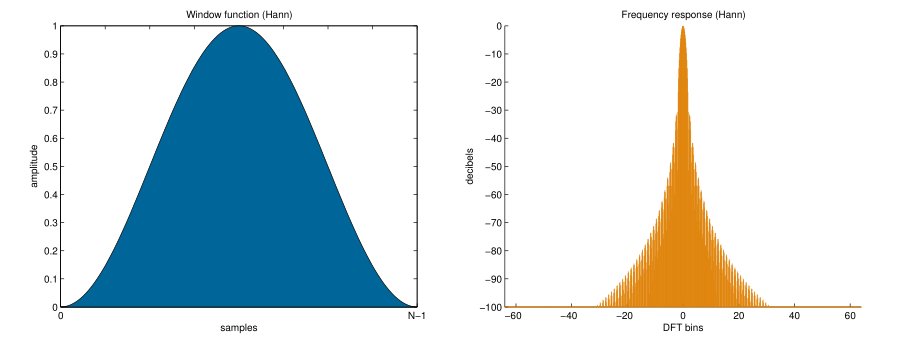
\includegraphics[width=0.4\paperwidth,valign=t]{hanning_window}%
            }
            \vfill
            \subfloat[Прозорец на Хеминг]{%
                \includegraphics[width=0.5\paperwidth,valign=t]{hamming_window}%
            }
        \caption{Често срещани прозоречни функции}%
        \label{fig:char:2}
    \end{figure}

    TODO: тука още приказки за прозорци. Прозорецът е моята врата и аз вървя към тях и ги разпитвам.

    След като фреймовете вече са периодични, на всеки от тях се прави фурие преобразувание. Може би тука за FFT. За да се почертае периодичносттадсгфгвегветгвег ГРРРР Чувствителността на човешкото ухо е различна в зависимост от честотата. Всъщност, скалата, по която чуваме звука, е по-скоро логаритмична. Мел скалата е изкуствено (емпрично) създадена, така че разликите между меловете да се усещат като еднакви. Връзката между меловете и честотите е логаритмична, като се задава с формулата:
    \begin{flalign*}
        & m = 2595 \log_{10}(1 + \frac{f}{100}) &&
    \end{flalign*}

    \begin{figure}[H]
        \centering
        \includegraphics[width=0.8\paperwidth]{mel_filterbank}%
        \caption{Мел}
        \label{fig:char:3}
    \end{figure}

    За да се изобрази спектъра в Мел скалата, се натрупват 


\end{document}